
\documentclass[a4paper,10pt]{article}


\usepackage{enumitem} % Pour personnaliser les listes
\usepackage[T1]{fontenc}
\usepackage{amsmath, amssymb} % Pour les mathématiques
\usepackage{xcolor} % Pour les couleurs
\usepackage{geometry} % Pour ajuster les marges
\usepackage{tikz}
\usetikzlibrary{automata, positioning}

% Configuration des marges
\geometry{
    a4paper,
    left=2cm,
    right=2cm,
    top=2cm,
    bottom=2cm
}

% Définition des couleurs
\definecolor{bleuclair}{rgb}{0.8, 0.9, 1}
\definecolor{rougeclair}{rgb}{1, 0.8, 0.8}
\definecolor{vertclair}{rgb}{0.8, 1, 0.8}
\definecolor{grisclair}{rgb}{0.9, 0.9, 0.9}
\definecolor{nouvellecouleur}{rgb}{1, 1, 0.7}

% Compteurs pour les sections numérotées
\newcounter{numdefinition}
\newcounter{numtheoreme}
\newcounter{numdemonstration}
\newcounter{numexemple}
\newcounter{numremarque}
\setcounter{numdefinition}{0}
\setcounter{numtheoreme}{0}
\setcounter{numdemonstration}{0}
\setcounter{numexemple}{0}
\setcounter{numremarque}{0}

% Commande pour les définitions
\newcommand{\definition}[2]{%
    \vspace{1em}%
    \stepcounter{numdefinition}%
    \noindent%
    \fcolorbox{black}{bleuclair}{%
        \parbox[t]{0.95\textwidth}{%
            \textbf{\sffamily Définition \thenumdefinition : #1} \par % Nom de la définition
            #2 % Contenu de la définition
        }%
    }%
    \vspace{1em}%
}

% Commande pour les théorèmes
\newcommand{\theoreme}[2]{%
    \vspace{1em}%
    \stepcounter{numtheoreme}%
    \noindent%
    \fcolorbox{black}{rougeclair}{%
        \parbox[t]{0.95\textwidth}{%
            \textbf{\sffamily Théorème \thenumtheoreme : #1} \par % Nom du théorème
            #2 % Contenu du théorème
        }%
    }%
    \vspace{1em}%
}

% Commande pour les démonstrations
\newcommand{\demonstration}[1]{%
    \vspace{1em}%
    \stepcounter{numdemonstration}%
    \noindent%
    \fcolorbox{black}{vertclair}{%
        \parbox[t]{0.95\textwidth}{%
            \textbf{\sffamily Démonstration \thenumdemonstration :} \par%
            #1%
        }%
    }%
    \vspace{1em}%
}

% Commande pour les exemples
\newcommand{\exemple}[2]{%
    \vspace{1em}%
    \stepcounter{numexemple}%
    \noindent%
    \fcolorbox{black}{grisclair}{%
        \parbox[t]{0.95\textwidth}{%
            \textbf{\sffamily Exemple \thenumexemple : #1} \par%
            #2%
        }%
    }%
    \vspace{1em}%
}


% Commande pour les remarques
\newcommand{\remarque}[2]{%
    \vspace{1em}%
    \stepcounter{numremarque}%
    \noindent%
    \fcolorbox{black}{nouvellecouleur}{%
        \parbox[t]{0.95\textwidth}{%
            \textbf{\sffamily Remarque \thenumremarque : #1} \par%
            #2%
        }%
    }%
    \vspace{1em}%
}


% Titre du document
\title{TIPE}
\author{T. Lestienne}
\date{}

\begin{document}

\maketitle%

\section{Formalisation de la cryptographie}

\definition{chiffre}{
    Un \textit{chiffre} défini sur $(\mathcal{K}, \mathcal{M}, \mathcal{C})$, avec $\mathcal{K}$ l'\textit{espace des clés}, $\mathcal{M}$ l'\textit{espace des messages}, et $\mathcal{C}$ l'\textit{espace des messages chiffrés}, est une paire $(E, D)$ telle que:
    \begin{itemize}[itemsep=1pt] % Réduction de l'espacement entre les items
        \item $E : \mathcal{K} \times \mathcal{M} \to \mathcal{C}$ est la fonction de chiffrement,
        \item $D : \mathcal{K} \times \mathcal{C} \to \mathcal{M}$ est la fonction de déchiffrement,
        \item $\forall m \in \mathcal{M}, \, \forall k \in \mathcal{K}, \, D(k, E(k, m)) = m$.
    \end{itemize}
}

\exemple{Application au code de César}{
    Le code de César consiste à associer à chaque lettre un nombre lié à sa position dans l'alphabet (voir tableau ci-dessous). Puis effectuer un décalage de $k$ "vers la droite".

    \[
    \begin{array}{|c|c|c|c|c|c|c|c|c|c|c|c|c|c|}
        \hline
        A & B & C & D & E & F & G & H & I & J & K & \cdots & Y & Z \\
        \hline
        0 & 1 & 2 & 3 & 4 & 5 & 6 & 7 & 8 & 9 & 10  & \cdots & 24 & 25 \\
        \hline
    \end{array}
    \]\\

    \textbf{Formellement :} Le chiffre de César est défini sur $(\mathcal{K}, \mathcal{M}, \mathcal{C})$ avec $\mathcal{K} = [|0;25|]$, $\mathcal{M} = \mathcal{C} = \{A, B, \dots, Z\}$.
    Les fonctions de chiffrement $E$ et de déchiffrement $D$ sont définies par :
    \[
    E : \left\{
    \begin{array}{ccc}
    \mathcal{K} \times \mathcal{M} & \to & \mathcal{C} \\
    (k, m) & \mapsto & (m + k) \mod 26
    \end{array}
    \right .
    \]

    \[
    D : \left\{
    \begin{array}{ccc}
    \mathcal{K} \times \mathcal{C} & \to & \mathcal{M} \\
    (k, c) & \mapsto & (c - k) \mod 26
    \end{array}
    \right .
    \]\\

    On a bien $\forall m \in \mathcal{M}, \, \forall k \in \mathcal{K}, \, D(k, E(k, m))= (m + k \mod 26) - k \mod 26 = m \mod 26 = m$\\

    \textbf{Application :} Chiffrement de TEST avec $k = 10$ :
    \begin{itemize}
        \item $T \to D$ \quad $(19 + 10) \mod 26 = 3$,
        \item $E \to O$ \quad $(4 + 10) \mod 26 = 14$,
        \item $S \to C$ \quad $(18 + 10) \mod 26 = 2$,
        \item $T \to D$ \quad $(19 + 10) \mod 26 = 3$.
    \end{itemize}
    Le message chiffré est donc $\text{DOCD}$.

    Pour le déchiffrement, on utilise $D(k, c)$ :
    \begin{itemize}
        \item $D \to T$ \quad $(3 - 10) \mod 26 = 19$,
        \item $O \to E$ \quad $(14 - 10) \mod 26 = 4$,
        \item $C \to S$ \quad $(2 - 10) \mod 26 = 18$,
        \item $D \to T$ \quad $(3 - 10) \mod 26 = 19$.
    \end{itemize}
    Le message déchiffré est donc $\text{TEST}$.
}

\remarque{}{deux occurences de la même lettre seront encoder par la même lettre}

\remarque{}{Dans ce cas, les fonctions $\mathcal{E}$ et $\mathcal{D}$ s'effectuent en $\mathcal{O}(1)$.}

\section{Formalisation des machines de Mealy}

\definition{Transducteur}{
    Un \textit{transducteur} est un sextuplet $ T = (\Sigma_1, \Sigma_2, Q, q_0, \delta) $
    tel que :
    \begin{itemize}[itemsep=1pt] % Réduction de l'espacement entre les items
        \item $ \Sigma_1 $ est l'alphabet d'entrée,
        \item $ \Sigma_2 $ est l'alphabet de sortie,
        \item $ Q $ est l'ensemble des états,
        \item $ q_0 \in Q $ est l'état initial,
        \item $ \delta : Q \times \Sigma_1 \to Q \times \Sigma_2 $ est la fonction de transition.
    \end{itemize}
}

\exemple{Representation graphique}{
    Le transducteur $T = (\{a,b,c\},\{0,1\},\{q_0,q_1,q_2\},q_0,\delta)$ Avec $\delta$
    \[\begin{array}{|c|c|c|c|}
        \hline
        \textbf{État actuel} & \textbf{Symbole lu} & \textbf{État suivant} & \textbf{Sortie} \\
        \hline
        q_0 & a & q_1 & 0 \\
        q_0 & b & q_0 & 1 \\
        q_1 & a & q_2 & 1 \\
        q_1 & c & q_0 & 0 \\
        q_2 & b & q_2 & 1 \\
        q_2 & a & q_0 & 1 \\
        q_2 & c & q_0 & 0 \\
        \hline
    \end{array}\]

    Peut être representé par

    \begin{center}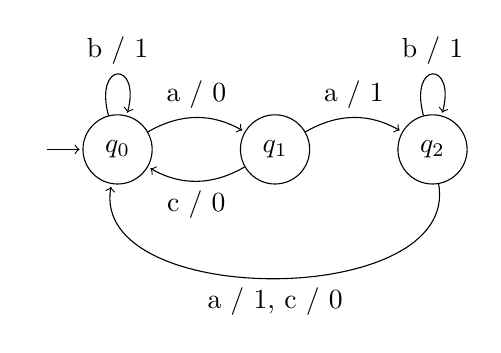
\begin{tikzpicture}[shorten >=1pt, node distance=2cm, on grid, auto]
        % Nœuds
        \node[state, initial, initial text={}] (q_0)   {$q_0$};
        \node[state] (q_1) [right=of q_0] {$q_1$};
        \node[state] (q_2) [right=of q_1] {$q_2$};

        % Flèches
        \path[->]
            (q_0) edge [loop above] node {b / 1} (q_0)
                edge [bend left] node {a / 0} (q_1)
            (q_1) edge [bend left] node {a / 1} (q_2)
                edge [bend left] node {c / 0} (q_0)
            (q_2) edge [loop above] node {b / 1} (q_2)
                edge [bend left=100] node {a / 1, c / 0} (q_0);
    \end{tikzpicture}\end{center}
}

\definition{Machine de Mealy}{
    une \textit{machine de mealy} $M = (\Sigma)$ est un transducteur tel que
}

\theoreme{}{
    Soit $\Sigma$ un alphabet et $N \in \mathbb{N}$ Il existe $(|\Sigma|! \times N^{|\Sigma|})^{|N|}$ Machines de Mealy a N états.
}

\demonstration{

    Ainsi il y a $(|\Sigma|! \times N^{|\Sigma|})^{|N|}$
}

\remarque{}{
    \centering
    \begin{tabular}{|c|c|}
        \hline
        & \\
        \( N \) & \((26! \times N^{26})^{|N|} \) \\
        \hline
        1 & $4.03 \times10^{26}$ \\
        2 & $7.32 \times10^{68}$ \\
        3 & $1.08 \times10^{117}$ \\
        4 & $1.09 \times10^{169}$ \\
        5 & $7.84 \times10^{223}$ \\
        \hline
    \end{tabular} % Ajout de cette ligne pour fermer le tableau correctement
}

\theoreme{}{
    Soit  \newline
    $A$ : Deux lettres successives dans le message original sont identique \newline
    $B$ : Deux lettres successives dans le message chiffré sont identique\newline\newline 
    $N = \frac{|\Sigma| \times P(A) - 1}{|\Sigma|\times P(B) - 1}$\newline

    }

\demonstration{ 
    $P (B\rvert A) = 1/N + \frac{N-1}{N} \times \frac{1}{|\Sigma|} $\newline \newline 
    $P (B \rvert \overline{A}) = \frac{N-1}{N} \times \frac{1}{|\Sigma|}$
    \newline\newline
    $P(B) = P(A) \times P(B|A) + P(\overline{A}) \times P(B|\overline{A})$\newline\newline
    $P(B) = (1/N + \frac{N-1}{N} \times \frac{1}{|\Sigma|}) * P(A) + 
            (\frac{N-1}{N} \times \frac{1}{|\Sigma|}) * P(\overline{A})$\newline\newline
    $P(B) = \frac{1}{N} \times P(A) + \frac{N-1}{N|\Sigma|}\times (P(A) + P(\overline{A}))$\newline\newline
    $P(B) = \frac{1}{N} \times P(A) + \frac{N-1}{N|\Sigma|}$\newline\newline
    $P(B) = \frac{N-1 + P(A)\times |\Sigma|}{N|\Sigma|}$\newline\newline
    $N|\Sigma|\times P(B) = N-1 + P(A)\times |\Sigma|$\newline\newline
    $N(|\Sigma|\times P(B) - 1) = P(A)\times |\Sigma| - 1$\newline\newline
    $N = \frac{|\Sigma| \times P(A) - 1}{|\Sigma|\times P(B) - 1}$\newline\newline
}

\remarque{synthese}{
    Soit $m$ un message sur $\Sigma$ et $k$ la clé choisie
    \[\begin{array}{|c|c|c|c|}
        \hline
        \textbf{Chiffre} & \textbf{Complexité} & \textbf{Complexité} & \textbf{Complexité de} \\
        & de E & de D & \textbf{l'attaque par force brute} \\
        \hline
        % Ajoutez ici les lignes du tableau
        \hline
    \end{array}\] % Ajout de cette ligne pour fermer le tableau correctement
}

%\remarque{}{}\\
%\definition{}{}\\
%\theoreme{}{}\\
%\demonstration{}{}\\
%\exemple{}{}

\end{document}
